\subsection{\label{subsec:FZV2}Plasmon modes}
\textbf{\textit{How do the field and charge carrier distributions of the plasmonic fundamental mode look like?}}\\
$\rightarrow$In the initial phase, we confine our focus to the examination of a localized particle plasmon, aiming 
to sidestep the description for volume or non-localized surface plasmons. Simply put, the particle plasmon arises from 
the interaction of free electrons in the conduction band of a particle with an electric field \cite{Anleitung}. 
This results in charge separation, and the ensuing Coulomb (restorative) force induces oscillation, with the fundamental 
mode being the dipole particle plasmon \cite{FZV2p3}. \\
The efficiency of mode excitation depends on the light frequency and polarization, with the light frequency 
ideally aligning with the resonance frequency of the considered mode, and the polarization being chosen in 
the direction of the mode's oscillation. The precise charge distribution and electric field rely on the shape 
of the nanoparticle, enabling targeted applications through the design of various forms \cite{FZV2p1}. 
For the first two modes, the electric field and the general charge distribution are outlined in Fig.~\ref{fig:moden}.
\begin{figure}[h!]
    \centering
    \subfloat[\centering Dipole]{{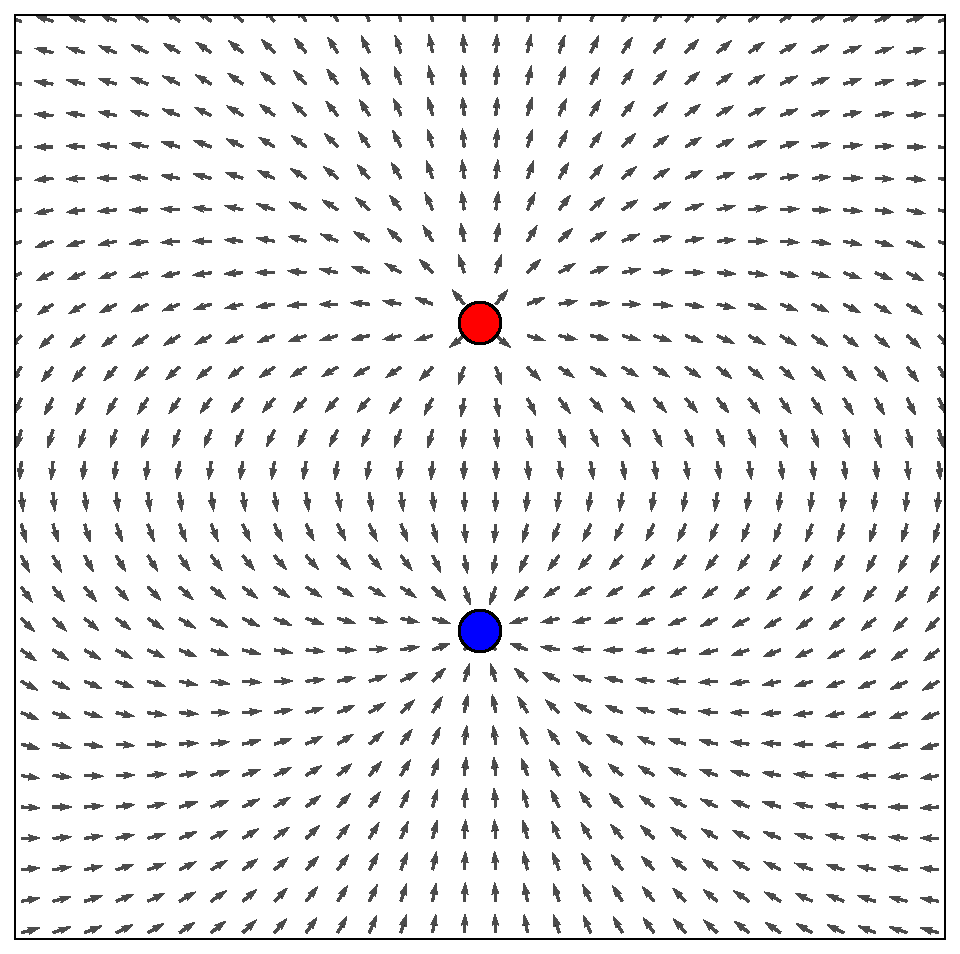
\includegraphics[width=0.45\textwidth]{c1.pdf} }}
    \qquad
    \subfloat[\centering Quadrupole]{{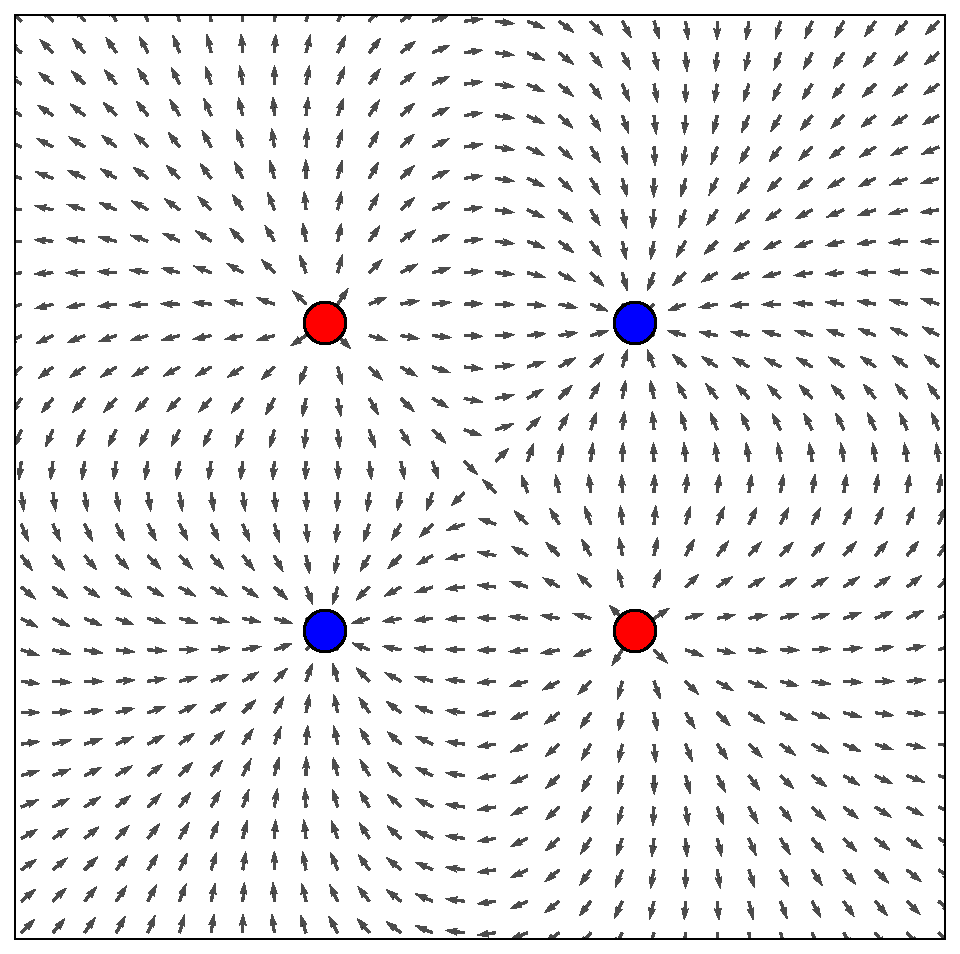
\includegraphics[width=0.45\textwidth]{c2.pdf} }}
    \caption{\label{fig:moden}Sketch of the electric field (black arrows) of a dipole and a quadrupole, 
    along with their respective charges (red=positive, blue=negative). 
    An electromagnetic wave can induce local charge separation within the nanoparticle, 
    generating an electric field. 
    The actual field depends on the shape of the nanoparticle and is therefore depicted very generally here.}
\end{figure}\FloatBarrier \,\\

\textbf{\textit{Describe why there are plasmon modes that cannot be excited under a microscope with laser light. 
Also, sketch the field and charge carrier distribution of such a mode. How can such a mode be excited nonetheless?}}\\
$\rightarrow$The next higher mode, the quadrupole particle plasmon, exhibits a more refined local charge separation. 
Excitation by laser light can be challenging as the oscillation direction differs from the dipole mode, and the mode's 
resonance frequency is altered. Additionally, attention must generally be paid to ensure that the plasmon being excited 
shares the same oscillation direction (coupled with the propagation direction) as the incident light. \\
For instance, longitudinal surface plasmons cannot be excited by transverse light waves \cite{FZV2p2}. 
Further multipole particle plasmons can be excited through appropriate shapes, incidence angles, polarization, 
and light frequencies. In contrast to narrowband laser light, illumination with white light allows for broader mode excitation. \\